\documentclass[11pt,wide]{article}

\usepackage[utf8]{inputenc}

\usepackage{graphicx} 

\usepackage{mathtools}
\usepackage{amsthm}
\usepackage{verbatim}
\usepackage{xcolor}

\usepackage{hyperref}

\usepackage{relsize}

\hypersetup{
    colorlinks=true,
    linkcolor=blue,
    filecolor=magenta,      
    urlcolor=cyan,
    citecolor=green,
    pdftitle={Sharelatex Example},
    bookmarks=true,
}

\newcommand\numeq[1]%
  {\stackrel{\scriptscriptstyle \mkern-1.5mu#1\mkern-1.5mu }{=}}

\newtheorem{thm}{Twierdzenie}
\newtheorem{remark}{Uwaga}
\newtheorem{lemat}{Lemat}
\newtheorem{wniosek}{Wniosek}
\newtheorem{definicja}{Definicja}
\newtheorem{ciekawostka}{Ciekawostka}
\newtheorem{przyklad}{Przykład}
\newtheorem{rysunek}{Rysunek}

\newtheorem{theorem}{Theorem}
\newtheorem{lemma}{Lemma}

% Marginesy
\topmargin=-0.45in
\evensidemargin=0in
\oddsidemargin=0in
\textwidth=6.5in
\textheight=9.0in
\headsep=0.25in

\title{RPiS - first task}
\date{Wrocław, April 12, 2020}
\author{Jakub Kuciński, Pratik Ghosal}

\begin{document}

\maketitle
\thispagestyle{empty} 
\tableofcontents


\section{Standard normal distribution}
Standard normal distribution of random variable $X$ is described by probability density function:
\begin{equation}
\displaystyle f(x) = \frac{1}{\sqrt{2 \cdot \pi}} \mathlarger{e^{\mathlarger{-\frac{x^2}{2}}}}
\end{equation}


\section{Cumulative distribution function}
For cumulative distribution function we get the expression:
\begin{equation}
\displaystyle \Phi (t) = \int_{-\infty}^t \frac{1}{\sqrt{2 \cdot \pi}} \mathlarger{e^{\mathlarger{-\frac{x^2}{2}}}} \mathop{dx} 
\end{equation}
This integral doesn't have representation in terms of elementary functions, so it's difficult to find it's exact value. In purpose of finding CDF there's need to calculate approximations of values of this integral, but computing it in infinity can be tricky, so it's better to find easier expression.

\begin{lemma}
\(\Phi (t) + \Phi (-t) = 1\).
\end{lemma}

\begin{proof}
\begin{equation}
\displaystyle \Phi (t) + \Phi (-t) = \int_{-\infty}^t f(x) \mathop{dx} + \int_{-\infty}^{-t} f(x) \mathop{dx}
\end{equation}
From evenness of $f(x)$ the equality
\begin{equation}
\displaystyle \int_{-\infty}^{-t} f(x) \mathop{dx} = \int_{t}^{+\infty} f(x) \mathop{dx}
\end{equation}
holds. Hence:
\begin{equation}
\displaystyle \Phi (t) + \Phi (-t) = \int_{-\infty}^t f(x) \mathop{dx} + \int_{t}^{+\infty} f(x) \mathop{dx} =  \int_{-\infty}^{+\infty} f(x) \mathop{dx} = 1
\end{equation}
\end{proof}
So from lemma 1. for $t\geq 0$ $\Phi (t)$ can be written as:
\begin{align}
\displaystyle \Phi (t) &= 1 - \Phi (-t) = 1 - \left(\Phi (-t) + \int_{-t}^0 f(x) \mathop{dx} \right) +  \int_{-t}^0 f(x) \mathop{dx} = \\
  &= 1 - \int_{-\infty}^0 f(x) \mathop{dx} + \int_{0}^{t} f(x)\mathop{dx} = 1 - \frac{1}{2} \int_{-\infty}^{+\infty} f(x)\mathop{dx} + \int_{0}^{t} f(x)\mathop{dx} = \\
  &= 1 - \frac{1}{2} + \int_{0}^{t} f(x)\mathop{dx} = \frac{1}{2} + \int_{0}^{t} f(x)\mathop{dx}
\end{align}
Similarly for $t<0$:
\begin{align}
\displaystyle \Phi (t) &= 1 - \Phi (-t) = 1 - \left(\frac{1}{2} + \int_{0}^{-t} f(x) \mathop{dx} \right) = \frac{1}{2} - \int_{0}^{-t} f(x) \mathop{dx}
\end{align}
So the problem of computing $\Phi (t)$ can be reduced to computing:
\begin{equation}
\displaystyle \int_0^t \frac{1}{\sqrt{2 \cdot \pi}} \mathlarger{e^{\mathlarger{-\frac{x^2}{2}}}}
\end{equation}
for $t>0$. As $\frac{1}{\sqrt{2 \cdot \pi}}$ is a constant, it is easier to just compute:
\begin{equation}
\displaystyle G(t) = \mathlarger{\int_0^t e^{\mathlarger{-\frac{x^2}{2}}}}
\end{equation}
and then multiplying it by $\frac{1}{\sqrt{2 \cdot \pi}}$.


\section{Computing CDF}
$G(t)$ for fixed $t$ is an integral over bounded range so it's possible to compute value of $G(t)$ by trapezoidal rule and reducing error by usage of Romberg method. By calculating integrals for $t$ in choosen range and with acceptably small intervals it's easy to draw a plot of CDF.

\begin{figure}[h!]
	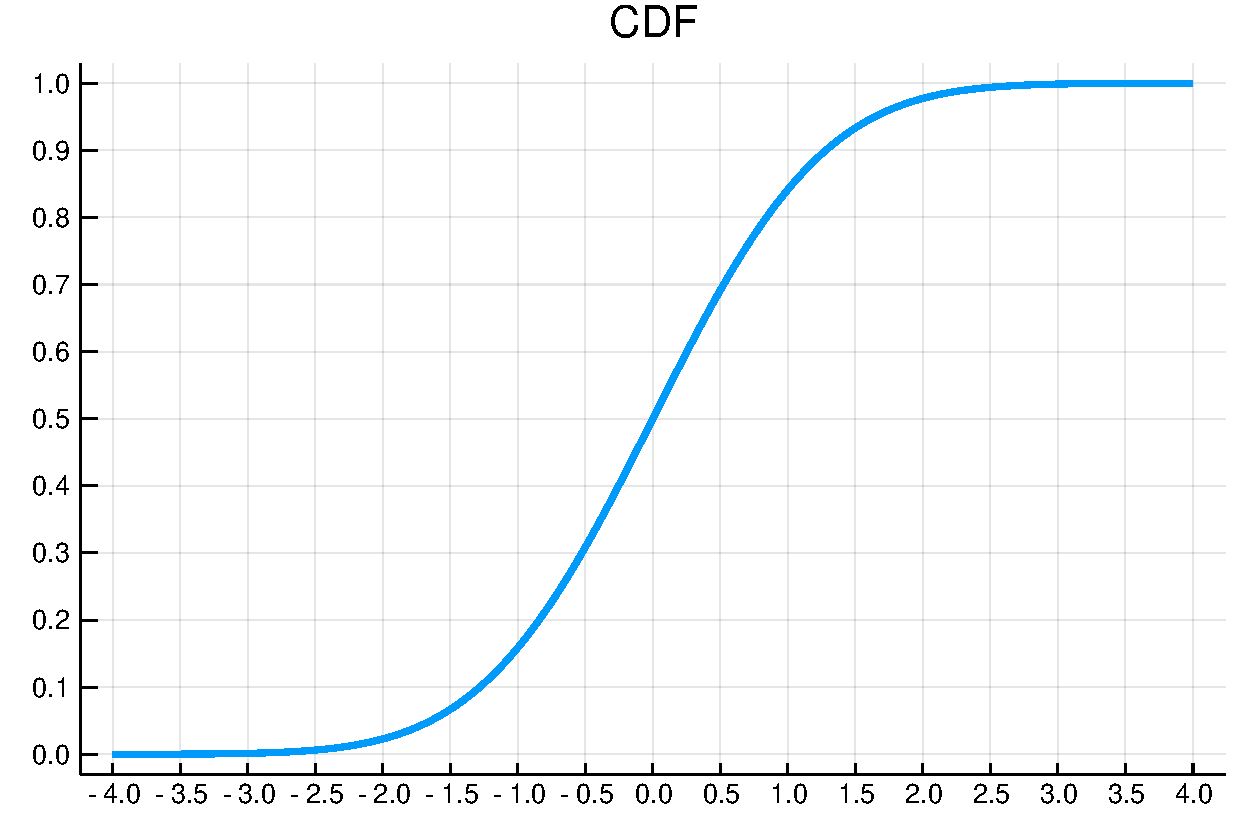
\includegraphics[width=160mm,scale=1.0]{cdf2}
\end{figure}
\end{document}